\section{Préparation de q-échantillon}

Étant donné un réseau bayésien discret, il est possible d'échantillonner la distribution de probabilité sous-jacente à l'aide d'un circuit quantique. En effet, cette méthode d'échantillonnage permet d'exploiter les avantages computationnels introduits par les algorithmes quantiques, notamment avec l'amplification d'amplitude, celle-ci détaillée dans les sections précédentes \cite{borujeni2021quantum}.

\subsection{Description}
La construction du circuit quantique se fait en trois principales étapes :
\begin{itemize}
\item[1] Associer chaque variable du réseau bayésien à un ou plusieurs qubits (en fonction du nombre de valeurs prises par la variable).
\item[2] Associer les probabilités marginales et conditionnelles de chaque variable aux amplitudes associées aux divers états des qubits.
\item[3] Assimiler les amplitudes des états quantiques en utilisant des portes de rotation (contrôlées), dans un ordre topologique du graphe $G$.
\end{itemize}
Dans un premier temps, nous nous contentons du cas binaire où les variables du réseau bayésien prennent seulement deux valeurs.
\\
Soit  $\mathcal{B} = (G,\mathcal{X})$ un réseau bayésien avec $G=(V,E)$ un graphe orienté acyclique et $\mathcal{X}=(X_i)_{i\in[\![1,k]\!]}$ une famille de variables aléatoires à valeurs dans $\{0,1\}$ définies sur $(\Omega, \mathcal{F}, \mathbb{P})$. On définit l'isomorphisme :
\begin{align*}
    \Psi : \mathcal{X} &\longrightarrow \mathbb{C}^2\\
    X_i &\longmapsto |\psi_i\rangle
\end{align*}
qui associe chaque variable du réseau bayésien à un vecteur d'état implémenté par un qubit du circuit. Nous représentons ainsi la famille $\mathcal{X}$ de variables aléatoires par un seul vecteur d'état à l'aide du produit tensoriel :
\[|\psi\rangle = \bigotimes_{i=1}^{k}|\psi_i\rangle \in (\mathbb{C}^2)^{\otimes k}\]
En pratique, les vecteurs $|\psi_i\rangle$\footnotemark \ sont initialisés à $|0\rangle$ lors de leur initialisation dans le circuit. Nous devons ainsi leur accorder les amplitudes appropriées afin d'obtenir les probabilités de la variable aléatoire lors de la mesure. Autrement dit, pour tout $i\in[\![1,k]\!]$, nous voulons obtenir :
\[|\psi_i\rangle = \alpha_i|0\rangle + \beta_i|1\rangle\]
avec $|\alpha_i|^2 = \mathbb{P}(X_i=0)$ et $|\beta_i|^2 = \mathbb{P}(X_i=1)$.
\footnotetext{Afin de simplifier les explications, par abus de langage, nous utiliserons indifféremment les termes "qubits" et "vecteurs d'état" et indifféremment les termes "portes quantiques" et "opérateurs unitaires".}
\\
On distingue deux cas :
\begin{itemize}
\item Les variables $X_i$ sans parents dans $G$ : Celles-ci sont traitées d'abord. Nous appliquons une porte de rotation $R_Y$ avec un angle $\theta$ pour associer les probabilités d'une variable aléatoire à son qubit représentant. La définition de $R_Y$ et le calcul de $\theta$ sont explicités dans la sous-section \ref{calcul_simple_rot}.
\item Les variables $X_i$ ayant des parents dans $G$ : Nous les traitons en second lieu dans un ordre topologique du graphe $G$. De plus, plusieurs angles devront être calculés pour les différentes rotations conditionnées par les valeurs prises par les parents. En effet, puisque les variables sont binaires, pour $|Pa(X_i)|=m_i$ nous avons $2^{m_i}$ rotations à déterminer et à appliquer sur le vecteur $|\psi_i\rangle$. Ces rotations sont implémentées par des portes de rotation contrôlées dont les angles dépendent des probabilités conditionnelles de $X_i$. Leur calcul est formulé dans la sous-section \ref{calcul_multi_rot}.
\end{itemize}

\subsection{Sphère de Bloch}
\label{section_Bloch}

\begin{figure}
\centering
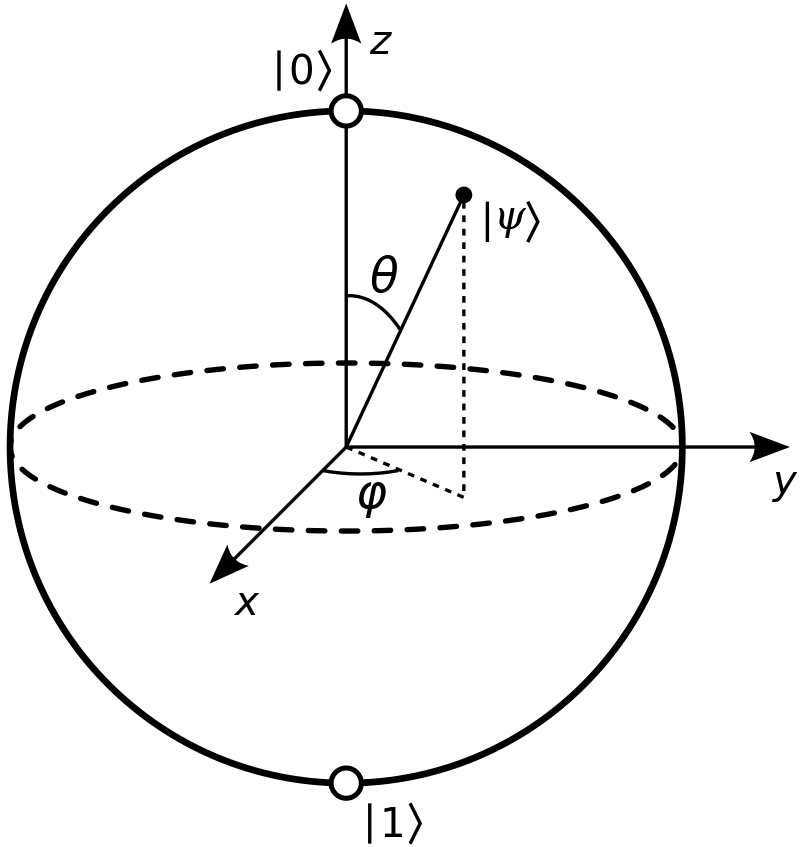
\includegraphics[scale=0.2]{Bloch_sphere}
\caption{La sphère de Bloch}
\label{fig:Bloch}
\end{figure}

Définissons au préalable la sphère de Bloch (Figure \ref{fig:Bloch}) qui permet d'illustrer les transformations des portes quantiques agissant sur un seul qubit, dont notamment celles de la porte $R_Y$.
\\
Considérons un état $|\psi \rangle =\alpha |0\rangle +\beta |1\rangle$ ayant pour amplitudes $\alpha ,\beta \in \mathbb{C}$ avec $|\alpha|^{2}+|\beta |^{2}=1$. En passant aux coordonnées polaires, il existe $r_{\alpha}, r_{\beta} \in \mathbb{R}_+$ et $\phi_{\alpha}, \phi_{\beta} \in [0,2\pi[$ tels que:
\[|\psi \rangle = r_{\alpha}e^{i\phi_{\alpha}}|0\rangle + r_{\beta}e^{i\phi_{\beta}} |1\rangle\]. 
\\
Or, sachant que $|re^{i\phi}|^2 = re^{i\phi}re^{-i\phi} = r^2$, on en deduit que la probabilite d'observation d'un qubit est entièrement déterminée par le module de son amplitude. On définit ainsi la relation d'équivalence $\sim$ sur $\mathbb{C}^2$ par $\alpha \sim \beta \iff |\alpha|^2=|\beta|^2$. Nous obtenons ainsi:
\[|\psi \rangle \sim r_{\alpha}|0\rangle + r_{\beta}e^{i(\phi_{\beta}-\phi_{\alpha})} |1\rangle\]
De plus, on remarque que $r_{\alpha}^2+r_{\beta}^2=1$ et donc $r_{\alpha}, r_{\beta} \in [0,1]$. Par conséquent, les points $(r_{\alpha}, r_{\beta})$ appartiennent au premier quadrant du cercle unité de $\mathbb{R}^2$. Il existe alors un unique $\theta \in [0,\pi]$ tel que $(r_{\alpha}, r_{\beta}) = (\mathrm{cos}(\theta/2),\mathrm{sin}(\theta/2))$. En posant $\phi = \phi_{\beta}-\phi_{\alpha} + 2n\pi$ avec $n \in \mathbb{Z}$ de sorte que $\phi \in [0,2\pi[$, on obtient finalement:
\[|\psi \rangle \sim \mathrm{cos}(\theta/2)|0\rangle + \mathrm{sin}(\theta/2)e^{i\phi}|1\rangle\]
Dans cette représentation, on a:
\[(1,0,0) \cong \frac{|0\rangle+|1\rangle}{\sqrt{2}}, \ (0,1,0) \cong \frac{|0\rangle+i|1\rangle}{\sqrt{2}}, \ (0,0,1) \cong |0\rangle\]
et en outre $|1\rangle \cong (0,0,-1)$.
\\
Le point remarquable de cette construction est le fait qu'elle nous permet d’étudier les qubits de $\mathbb{C}^2$ sous la structure algébrique de $\mathbb{R}^3$ en utilisant les coordonnées sphériques. En effet, sachant que l'illustration graphique d'un nombre complexe se fait sur un plan de dimention 2, la sphère de Bloch nous permet de visualiser des transformation de 4 dimentions en utilisant seulement 3 grâce a la relation d'équivalence définie auparavant. 

\subsection{Rotation pour les variables sans parents}
\label{calcul_simple_rot}
En étant muni de la sphère de Bloch, la porte $R_Y(\theta)$ donnée sous sa forme matricielle par
\begin{align*}
R_Y(\theta) = 
\begin{bmatrix}
\mathrm{cos}(\theta/2) & -\mathrm{sin}(\theta/2) \\
\mathrm{sin}(\theta/2) & \mathrm{cos}(\theta/2)
\end{bmatrix}
\end{align*}
effectue une rotation autour l'axe Y de la sphère d'un angle de $\theta$ (d'où le nom $R_Y$). 
Sachant qu'un qubit est initialisé à l'état $|0\rangle$ au début du circuit, en lui appliquant la porte $R_Y$, on se retrouve avec:
\[R_Y|0\rangle = \mathrm{cos}(\theta/2)|0\rangle+\mathrm{sin}(\theta/2)|1\rangle\]
Les probabilités associées aux états $|0\rangle$ et $|1\rangle$ sont donc $\mathrm{cos}^2(\theta/2)$ et $\mathrm{sin}^2(\theta/2)$ respectivement. Étant donnée une variable aléatoire $X_i$ sans parent dans $G$, nous voulons:
\[
\begin{cases}
\mathrm{cos}^2(\theta_{X_i}/2) = \mathbb{P}(X_i=0) \\
\mathrm{sin}^2(\theta_{X_i}/2) = \mathbb{P}(X_i=1)
\end{cases}
\]
On obtient alors en résolvant le système:
\[
\theta_{X_i} = 
 \begin{cases}
 2\times\mathrm{arctan}\left(\sqrt{\frac{\displaystyle \mathbb{P}(X_i=1)}{\displaystyle \mathbb{P}(X_i=0)}}\right) & \mathrm{pour} \ \mathbb{P}(X_i=0) \in \ ]0,1] \\
 \hfil \pi & \mathrm{pour} \ \mathbb{P}(X_i=0)=0
 \end{cases}
\]
La valeur $\theta_{X_i}$ est donc l'angle adéquat de rotation pour la porte $R_Y$ afin d'accorder les probabilités de $X_i$ au vecteur d'état $|0\rangle$. Sachant que les $X_i$ n'ont pas de parents dans $G$, nous pouvons direcetment accorder les amplitudes calculées à leur qubit représentatif. C'est donc pour cette raison qu'ils sont donc traités en premier. 

\subsection{Rotation pour les variables avec parents}
\label{calcul_multi_rot}
De la même manière, pour $X_i$ ayant des parents dans $G$, notons $\Pi_{X_i}$ les valeurs prises par les parents de $X_i$, nous avons:
\[
\theta_{X_i,\Pi_{X_i}} = 
2\times\mathrm{arctan}\left(\sqrt{\frac{\displaystyle \mathbb{P}(X_i=1|Pa(X_i)=\Pi_{X_i})}{\displaystyle \mathbb{P}(X_i=0|Pa(X_i)=\Pi_{X_i})}}\right) 
\]
pour $\mathbb{P}(X_i=0|Pa(X_i)=\Pi_{X_i}) \in \ ]0,1]$, et
$\theta_{X_i,\Pi_{X_i}} =  \pi$ quand cette probabilité est nulle.
\\
Ici $\theta_{X_i,\Pi_{X_i}}$ est l'angle de rotation permettant d'accorder les probabilités de $X_i$ conditionnées aux valeurs $\Pi_{X_i}$ prises par les parents de $X_i$. Cependant, une directe application de la porte $R_Y$ n'est pas convenable, il faut de plus conditionner $R_Y$ aux qubits représentant les variable de $Pa(X_i)$.
Cela nous amène aux portes de rotation contrôlées.
\\
Pour $U$ une porte quantique, nous définissons la porte $U$ contrôlée notée $CU$ agissant sur deux qubits par la matrice:
\[CU =
\left[
\begin{array}{cccc}
    1 & 0 & 0 & 0 \\
    0 & 1 & 0 & 0 \\
    0 & 0 & \multicolumn{2}{c}{\smash{\raisebox{-.5\normalbaselineskip}{$U$}}} \\
    0 & 0 &  & 
\end{array}
\right]
\in \mathcal{M}_{4}(\mathbb{C})
\]
Pour un vecteur d'état $|\psi\rangle$, l'application de $CU$ aux produits tensoriaux à gauche de $|\psi\rangle$ avec les états $|0\rangle$ et $|1\rangle$ nous donne:
\begin{align*}
CU (|0\rangle \otimes |\psi\rangle) =&\ |0\rangle \otimes |\psi\rangle \\
CU (|1\rangle \otimes |\psi\rangle) =&\ |1\rangle \otimes U|\psi\rangle 
\end{align*}
Ici, le qubit $|x\rangle$ pour $x\in\{0,1\}$ agit comme contrôle de la porte $U$ sur le qubit cible $|\psi\rangle$. En effet, on remarque que $CU$ n'applique les trasformations de $U$ sur $|\psi\rangle$ que si $|x\rangle = |1\rangle$. Sinon, pour $|x\rangle = |0\rangle$, le qubit $|\psi\rangle$ reste inchangé. On notera aussi que $CU$ ne réalise aucune transformation sur $|x\rangle$. 
\\
Plus généralement, pour $n\in\mathbb{N}^*$, la porte $C^nU$ agit sur $n$ qubits de contrôle et $1$ qubit cible. Sa représentation matricielle est donnée par la matrice par bloc:
\[C^nU =
\left[
\begin{array}{cccc}
    I_2 & 0 & \hdots & 0 \\
    0 & \ddots & \ddots & \vdots \\
    \vdots & \ddots & I_2 & 0 \\
    0 & \hdots & 0 & U
\end{array}
\right]
\in \mathcal{M}_{2(n+1)}(\mathbb{C})
\]
avec $0, \ I_2 \in \mathcal{M}_2(\mathbb{C})$ la matrice nulle et la matrice identité respectivement. 
\\
Étant donné le vecteur d'état $|c_1 \hdots c_n\rangle \otimes |\psi\rangle$ à $n+1$ qubits , avec $(|c_i\rangle)_{i\in[\![1,n]\!]}$ les qubits de contrôle et $|\psi\rangle$ le qubit cible, on a:
\[C^nU(|c_1 \hdots x_n\rangle \otimes |\psi\rangle) = |c_1 \hdots c_n\rangle \otimes U|\psi\rangle \iff \forall i \in [\![1,n]\!], \ |c_i\rangle = |1\rangle \]
C'est-à-dire que la porte $C^nU$ realise l'operation $U$ sur $|\psi\rangle$ si et seulement si \textit{tous} les qubits de contrôle $|c_i\rangle$ valent $|1\rangle$. 
Dans notre cas, une rotation contrôlée $C^{m_i}RY(\theta_{X_i, \Pi_{X_i}})$ agit sur le vecteur $|c_1 \hdots c_{m_i}\rangle \otimes |\psi_i\rangle$, avec $|\psi_i\rangle$ le qubit représentatif de la variable $X_i$, et $(|c_i\rangle)_{i\in[\![1,m_i]\!]}$ les qubits représentatifs des variables de $ Pa(X_i)$.
\\
Muni de la porte $C^{m_i}RY(\theta_{X_i, \Pi_{X_i}})$, nous somme en meseure d'accorder les amplitudes correspondantes. Cependant, sachant que les probabilités sont conditionnées par les valeurs $\Pi_{X_i}$, et que les portes contrôlées ne prennent effet que lorsque tous  les qubits de contrôle valent 1, nous devons par ailleurs transformer les qubits initialisés avant rotations à $|0\rangle$ en $|1\rangle$ avant le passage de $C^{m_i}RY(\theta_{X_i, \Pi_{X_i}})$, et les reconvertir dans leurs état de départ après.
En effet, nous voulons que $C^{m_i}RY(\theta_{X_i, \Pi_{X_i}})$ prenne effet dès lorsque $Pa(X_i)=\Pi_{X_i}$, il s'agit donc de trouver une porte $B_{\Pi_{X_i}}$ agissant sur $|c_1 \hdots c_{m_i}\rangle$ tel que:
\[
B_{\Pi_{X_i}}|c_1 \hdots c_{m_i}\rangle = |1\rangle^{\otimes m_i} \quad \mathrm{pour} \quad (c_1,\hdots,c_{m_i}) = \Pi_{X_i}
\]
\\
Pour cela, nous faisons recours à la porte $NOT$ donnée par:
\begin{align*}
NOT =
\left[
\begin{array}{cc}
    0 & 1 \\
    1 & 0
\end{array}
\right]
\in \mathcal{M}_{2}(\mathbb{C}) 
\end{align*}
où $NOT|0\rangle = |1\rangle$ et $NOT|1\rangle = |0\rangle$. 
La porte $B_{\Pi_{X_i}}$ s'exprime alors par le produit tensoriel:
\[B_{\Pi_{X_i}} = \bigotimes_{k \in \Pi_{X_i}} NOT^{1-k} \]
On a utilisé ici le fait que $\Pi_{X_i} \in \{0,1\}^{m_i}$ et que $NOT^0 = I_2$. 
\\
Finalement, l'opérateur décrivant les actions de toute les portes aboutissant à la mise en place des amplitude d'une variable $X_i$ avec parent conditionnées aux valeurs $\Pi_{X_i}$ est donné par: 
\[
\big(B_{\Pi_{X_i}} \!\! \otimes I_2 \big)
\big(C^{m_i}RY(\theta_{X_i, \Pi_{X_i}})\big)
\big(B_{\Pi_{X_i}} \!\! \otimes I_2 \big)
\]
Cette opération est ensuite répétée pour toutes les combinaisons possibles des valeurs $\Pi_{X_i}$ prises par les variables $Pa(X_i)$, donc $2^{m_i}$ fois comme mentionné auparavant.

\subsection{Représentation de variables discrètes à plus de deux valeurs}
\label{QBNgeneral}
Pour les variables aléatoires discrètes finies prenant un nombre quelconque de valeurs, il's'agit de discrétiser ces valeurs et d'utiliser plusieurs qubits pour représenter une seule variable. Plus précisément, pour $X_i \in \mathcal{X}$, $N_i = |X_i(\Omega)|$ nous utilisons $n_i = \lceil \mathrm{log}_2(N_i) \rceil$ qubits. En reprenant l'isomorphisme défini dans la section \ref{part1}, on a $\Phi_i:[\![0,N_i-1]\!] \rightarrow (\mathbb{C}^2)^{\otimes n_i}$ qui réalise cette association. 
Ainsi, le vecteur d'état représentant $X_i$ est donné par:
\[|\psi_i\rangle = \sum_{x=0}^{N_i-1}\alpha_{i,x}|x\rangle\]
où $|x\rangle = \Phi_i(x)$ et $|\alpha_{i,x}|^2 = \mathbb{P}(X_i=x)$. 
\\
Les rotations s'avèrent plus délicates dans le cadre général car elles se portent sur de multiples qubits. Nous devons alors procéder par étape, en se concentrant sur un qubit à la fois. 
Nous expliciterons par la suite le vecteur d'état $|x\rangle \in (\mathbb{C}^2)^{\otimes n_i}$ avec le produit tensoriel des qubits $|q_i\rangle \in \mathbb{C}^2$:
\[|q_1 \hdots q_{n_i}\rangle = |B(x,n_i)\rangle = |x\rangle \]
Dans un premier temps, notons $U_{X_i, [\![1,n_i]\!]}$ la porte de rotation recherchée qui agit sur $n_i$ qubits de sorte que:
\[U_{X_i, [\![1,n_i]\!]}|0\rangle^{\otimes n_i} = |\psi_i\rangle\]
Le principe est de trouver une décomposition de $U_{X_i, [\![1,n_i]\!]}$ en fonctions de $C^nRY$ et $NOT$. 
\\
Afin de simplifier les notations, nous omettrons l'indice $X_i$ de  $U_{X_i, [\![1,n_i]\!]}$ indiquant qu'il s'agit de la rotation concernant la variable $X_i$. La première étape de décomposition se présente ainsi:
\[U_{[\![1,n_i]\!]} = (B_{q_1} \cdot CU_{[\![2,n_i]\!],q_1=0} \cdot B_{q_1})(CU_{[\![2,n_i]\!],q_1=1})(RY(\theta_{q_1})\otimes I_2^{\otimes (n_i-1)})\]
Où $B_{q_1} = NOT \otimes I_2^{\otimes (n_i-1)}$ est la porte $NOT$ appliquée uniquement au premier qubit $|q_1\rangle$, et $CU_{[\![2,n_i]\!],q_1=1}$ la porte de rotation agissant sur les qubits $(|q_i\rangle)_{i\in[\![2,n_i]\!]}$, conditionnée avec $|q_1\rangle=|1\rangle$ et contrôlée par le qubit $|q_1\rangle$. La porte $CU_{[\![2,n_i]\!],q_1=0}$ est définie analoguement. 
\\
L'idée ici est de s'inspirer de la sous-section précédente concernant les rotations pour les variables avec parents pour effectuer une binarisation de la variable discrète.
\\
Calculons d'abord $\theta_{q_1}$, l'angle de rotation permettant à $R_Y$ d'accorder les amplitudes du premier qubit $|q_1\rangle$, avec $q_1$ le premier élément de $B(x,n_i)$. On défini la fonction indicatrice:
\begin{align*}
    \mathbbm{1}_{q_1} : {\{0,1\}}^{n_i} &\longrightarrow \{0,1\} \\
    (q_1, \hdots ,q_{n_i}) &\longmapsto
 \begin{cases}
 1 \ \mathrm{si} \ q_1 = 1 \\
 0 \ \mathrm{si} \ q_1 = 0 
 \end{cases}
\end{align*}
La valeur de rotation $\theta_{q_1}$ du premier qubit représentant $X_i$ est alors donnée par:
\begin{align*}
    \theta_{q_1} = 2\times\mathrm{arctan}\left[\sqrt{\frac{\displaystyle \mathbb{P}(\mathbbm{1}_{q_1}(B(X_i,n_i))=1)}{\displaystyle \mathbb{P}(\mathbbm{1}_{q_1}(B(X_i,n_i))=0)}}\right] \footnotemark
\end{align*}
\footnotetext{Par abus de notation nous pouvons voir cela comme $2\times\mathrm{arctan}\left[\sqrt{\frac{\displaystyle \mathbb{P}(q_1=1)}{\displaystyle \mathbb{P}(q_1=0)}}\right]$. }
En sommant sur $X_i(\Omega)$ on obtient:
\begin{align*}
    \mathbb{P}(\mathbbm{1}_{q_1}(B(X_i,n_i))=1) =&\ \sum_{x=0}^{N_i-1}\mathbb{P}(X_i=x)\mathbb{P}(\mathbbm{1}_{q_1}(B(X_i,n_i))=1|X_i=x) \\
    =&\ \sum_{x=0}^{N_i-1}\mathbb{P}(X_i=x)\mathbbm{1}_{q_1}(B(X_i,n_i)) \\
    =&\ \sum_{x=0}^{N_i-1}|\alpha_{i,x}|^2\mathbbm{1}_{q_1}(B(X_i,n_i))
\end{align*}
Enfin en utilisant le fait que les deux événements sont complémentaires nous obtenons: 
\begin{align*}
    \theta_{q_1} = 2\times\mathrm{arctan}\left[\sqrt{\frac{\displaystyle \sum_{x=0}^{N_i-1}|\alpha_{i,x}|^2\mathbbm{1}_{q_1}\left(B(x,n_i)\right)}{\displaystyle 1-\sum_{x=0}^{N_i-1}|\alpha_{i,x}|^2\mathbbm{1}_{q_1}\left(B(x,n_i)\right)}}\right]
\end{align*}
Une fois la rotation du premier qubit établie, nous utilisons le  même procédé pour décomposer les portes $CU_{[\![2,n_i]\!],q_1=1}$ et $CU_{[\![2,n_i]\!],q_1=0}$. 
\\
De manière générale, pour $j\in[\![1,n_i-2]\!]$, la porte de rotation $C^jU_{[\![j+1,n_i]\!], (q)_j=(x)_j}$ agissant sur les qubits $(|q_i\rangle)_{i\in[\![j+1,n_i]\!]}$ conditionnée avec le mot\footnotemark \ $\mathcal{S}_j \in \{0,1\}^j$ et contrôlée par les qubits représentant $\mathcal{Q}_j=(q_i)_{i\in[\![1,j]\!]}$ se décompose par la formule de récurrence suivante:
\footnotetext{Ici le terme "mot" est employé dans le contexe de language formel, en particulier $\mathcal{S}_j = s_1 \cdots s_j$ est un mot de longueur $j$ dans l'alphabet $\{0,1\}$. On utilise en outre la notation $\mathcal{Q}_j$ pour désigner le $j$-uplet $(q_1,\hdots,q_j)$. Enfin, $\mathcal{S}_j \cdot 0$ est le mot $\mathcal{S}_j$ concaténé avec la lettre $0$.} 
\[
C^jU_{[\![j+1,n_i]\!], \mathcal{Q}_j=\mathcal{S}_j} = U_0 \cdot U_1 \cdot [C^jRY(\theta_{q_{j+1}, \mathcal{Q}_j=\mathcal{S}_j})\otimes I_2^{\otimes (n_i-1-j)}]
\]
avec
\begin{align*}
U_0 =&\ C^jB_{q_{j+1}} \cdot C^{j+1}U_{[\![j+2,n_i]\!], (\mathcal{Q}_j\cdot q_{j+1})=(\mathcal{S}_j \cdot 0)} \cdot  C^jB_{q_{j+1}}  \\
U_1 =&\ \ \qquad \qquad C^{j+1}U_{[\![j+2,n_i]\!], (\mathcal{Q}_j\cdot q_{j+1})=(\mathcal{S}_j \cdot 1)}
\end{align*}
et 
$C^jB_{q_{j+1}} = C^jNOT \otimes I_2^{\otimes (n_i-1-j)}$. 
Ici, $\theta_{q_{j+1}, \mathcal{Q}_j=\mathcal{S}_j}$ se calcule avec la fonction indicatrice:
\begin{align*}
    \mathbbm{1}_{q_{j+1}, \mathcal{Q}_j=\mathcal{S}_j} : {\{0,1\}}^{n_i} &\longrightarrow \{0,1\} \\
    (q_1, \hdots ,q_{n_i}) &\longmapsto
 \begin{cases}
 1 \ \mathrm{si} \ q_{j+1} = 1 \ \mathrm{et} \ \mathcal{Q}_j=\mathcal{S}_j\\
 0 \ \mathrm{sinon}
 \end{cases}
\end{align*}
On a:
\begin{align*}
    \theta_{q_{j+1}, \mathcal{Q}_j=\mathcal{S}_j} =&\ 2\times\mathrm{arctan}\left[\sqrt{\frac{\displaystyle \mathbb{P}(\mathbbm{1}_{q_{j+1}}(B(X_i,n_i))=1|\mathbbm{1}_{\mathcal{Q}_j=\mathcal{S}_j}(B(X_i,n_i))=1)}{\displaystyle \mathbb{P}(\mathbbm{1}_{q_{j+1}}(B(X_i,n_i))=0|\mathbbm{1}_{\mathcal{Q}_j=\mathcal{S}_j}(B(X_i,n_i))=1)}}\right] \\
    =&\ 2\times\mathrm{arctan}\left[\sqrt{\frac{\displaystyle \mathbb{P}(\mathbbm{1}_{q_{j+1}, \mathcal{Q}_j=\mathcal{S}_j}(B(X_i,n_i))=1)}{\displaystyle \mathbb{P}(\mathbbm{1}_{q_{j+1}, \mathcal{Q}_j=\mathcal{S}_j}(B(X_i,n_i))=0)}}\right] \\
    =&\ 2\times\mathrm{arctan}\left[\sqrt{\frac{\displaystyle \sum_{x=0}^{N_i-1}|\alpha_{i,x}|^2\mathbbm{1}_{q_{j+1}, \mathcal{Q}_j=\mathcal{S}_j}\left(B(x,n_i)\right)}{\displaystyle 1-\sum_{x=0}^{N_i-1}|\alpha_{i,x}|^2\mathbbm{1}_{q_{j+1}, \mathcal{Q}_j=\mathcal{S}_j}\left(B(x,n_i)\right)}}\right]
\end{align*}
Pour $N_i=|X_i(\Omega)|$ cette construction utilise $2^{\lceil \mathrm{log}_2(N_i) \rceil}-1$ portes $C^nRY$ et $2^{\lceil \mathrm{log}_2(N_i) \rceil}-2$ portes $C^nNOT$.
Le nombre total de portes quantiques utilisées est donc majoré par :
\[\sum_{\substack{X_i \in \mathcal{X} \\ N_i = |X_i(\Omega)|}}
\left[
2^{\lceil \mathrm{log}_2(N_i)\rceil+1} \prod_{\substack{X_j\in Pa(X_i) \\ N_j = |X_j(\Omega)|}}N_j 
\right] 
\]
En particulier pour un réseau bayésien binaire à $k$ variables, posons $m = \underset{X_i\in\mathcal{X}}{\mathrm{max}}(|Pa(X_i)|)$ le degré entrant maximale.  La complexité calculée en nombre de portes quantiques est de $\mathcal{O}(k2^m)$.
